%%%%%%%%%%%%%%%%%%%%%%%%%%%%%%%%%%%%%%%%%%%%%%%%%%%%%%%%%%%%%%%%
% Sim
%%%%%%%%%%%%%%%%%%%%%%%%%%%%%%%%%%%%%%%%%%%%%%%%%%%%%%%%%%%%%%%%
\section{仿真}
可以用上一节中推导出的式\eqref{eqModelTotal}建立被控对象微分方程,
也可以建立向量形式的微分方程
\begin{align}
    \ddot{\vec{r}} = \frac{\mu}{|\vec{r}|^3}\vec{r}+\vec{L}+\vec{D} \label{eqSim1}
\end{align}
其中阻力向量为
\begin{align}
    \vec{D} = -D\frac{\vec{v}}{|\vec{v}|} \label{eqSim2}
\end{align}
升力向量$\vec{L}$与铅垂面夹角为倾侧角$\sigma$,
为了能将$\vec{L}$用其他已知向量表示,
需要构造一对与$\vec{L}$同平面的正交单位向量。
当速度向量$\vec{v}$已知时,
定义一个垂直于地面的法向量$\vec{n}=[0,0,1]^\text{T}$,
则$\vec{V}$与$\vec{n}$张成铅垂面,
另构造一个垂直于铅垂面的单位向量$\vec{n}_2$,
和另一个与$\vec{n}_2$和$\vec{v}$都垂直且方向向上的单位向量$\vec{n}_1$,
则$\vec{n}_1$位于铅垂面内,
此时$\vec{L}$与$\vec{n}_1$的夹角即为倾侧角,
$\vec{n}_1$和$\vec{n}_2$即为用于表示$\vec{L}$的正交单位向量,
即
\begin{align}
    \vec{L}=\vec{n}_1\cos\sigma + \vec{n}_2\sin\sigma \label{eqSim3}
\end{align}
$\vec{n}_1$和$\vec{n}_2$的表达式为
\begin{align*}
    \vec{n}_2 =& \frac{\vec{v}\times\vec{n}}{||\vec{v}\times\vec{n}||} \\
    \vec{n}_1 =& \frac{\vec{n}_2\times\vec{v}}{||\vec{n}_2\times\vec{v}||}
\end{align*}
微分方程式\eqref{eqSim1}\eqref{eqSim2}\eqref{eqSim3}共同组成被控对象模型。
建立飞行器被控对象模型的模块框图如图\ref{figSimPlant}所示。
\begin{center}
	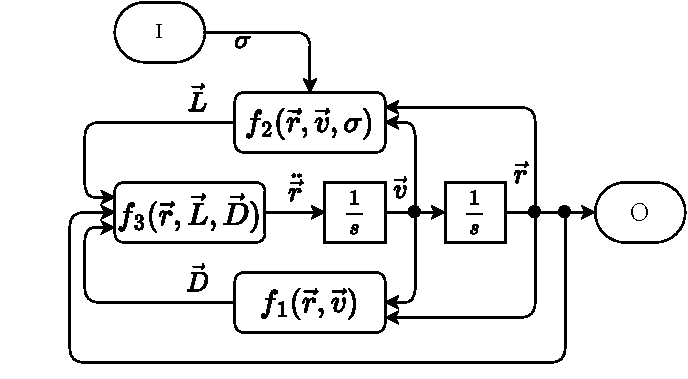
\includegraphics[scale=0.8]{plant.pdf}  \\
	\figcaption{被控对象模型的模块框图}\label{figSimPlant}
\end{center}
图中,被控对象的输入(控制量)为倾侧角$\sigma$,
输出为位置$\vec{r}$。


